\documentclass{article}\usepackage[]{graphicx}\usepackage[]{xcolor}
% maxwidth is the original width if it is less than linewidth
% otherwise use linewidth (to make sure the graphics do not exceed the margin)
\makeatletter
\def\maxwidth{ %
  \ifdim\Gin@nat@width>\linewidth
    \linewidth
  \else
    \Gin@nat@width
  \fi
}
\makeatother

\definecolor{fgcolor}{rgb}{0.345, 0.345, 0.345}
\newcommand{\hlnum}[1]{\textcolor[rgb]{0.686,0.059,0.569}{#1}}%
\newcommand{\hlsng}[1]{\textcolor[rgb]{0.192,0.494,0.8}{#1}}%
\newcommand{\hlcom}[1]{\textcolor[rgb]{0.678,0.584,0.686}{\textit{#1}}}%
\newcommand{\hlopt}[1]{\textcolor[rgb]{0,0,0}{#1}}%
\newcommand{\hldef}[1]{\textcolor[rgb]{0.345,0.345,0.345}{#1}}%
\newcommand{\hlkwa}[1]{\textcolor[rgb]{0.161,0.373,0.58}{\textbf{#1}}}%
\newcommand{\hlkwb}[1]{\textcolor[rgb]{0.69,0.353,0.396}{#1}}%
\newcommand{\hlkwc}[1]{\textcolor[rgb]{0.333,0.667,0.333}{#1}}%
\newcommand{\hlkwd}[1]{\textcolor[rgb]{0.737,0.353,0.396}{\textbf{#1}}}%
\let\hlipl\hlkwb

\usepackage{framed}
\makeatletter
\newenvironment{kframe}{%
 \def\at@end@of@kframe{}%
 \ifinner\ifhmode%
  \def\at@end@of@kframe{\end{minipage}}%
  \begin{minipage}{\columnwidth}%
 \fi\fi%
 \def\FrameCommand##1{\hskip\@totalleftmargin \hskip-\fboxsep
 \colorbox{shadecolor}{##1}\hskip-\fboxsep
     % There is no \\@totalrightmargin, so:
     \hskip-\linewidth \hskip-\@totalleftmargin \hskip\columnwidth}%
 \MakeFramed {\advance\hsize-\width
   \@totalleftmargin\z@ \linewidth\hsize
   \@setminipage}}%
 {\par\unskip\endMakeFramed%
 \at@end@of@kframe}
\makeatother

\definecolor{shadecolor}{rgb}{.97, .97, .97}
\definecolor{messagecolor}{rgb}{0, 0, 0}
\definecolor{warningcolor}{rgb}{1, 0, 1}
\definecolor{errorcolor}{rgb}{1, 0, 0}
\newenvironment{knitrout}{}{} % an empty environment to be redefined in TeX

\usepackage{alltt}
\usepackage{amsmath} %This allows me to use the align functionality.
                     %If you find yourself trying to replicate
                     %something you found online, ensure you're
                     %loading the necessary packages!
\usepackage{amsfonts}%Math font
\usepackage{graphicx}%For including graphics
\usepackage{hyperref}%For Hyperlinks
\usepackage[shortlabels]{enumitem}% For enumerated lists with labels specified
                                  % We had to run tlmgr_install("enumitem") in R
\hypersetup{colorlinks = true,citecolor=black} %set citations to have black (not green) color
\usepackage{natbib}        %For the bibliography
\setlength{\bibsep}{0pt plus 0.3ex}
\bibliographystyle{apalike}%For the bibliography
\usepackage[margin=0.50in]{geometry}
\usepackage{float}
\usepackage{multicol}

%fix for figures
\usepackage{caption}
\newenvironment{Figure}
  {\par\medskip\noindent\minipage{\linewidth}}
  {\endminipage\par\medskip}
\IfFileExists{upquote.sty}{\usepackage{upquote}}{}
\begin{document}

\vspace{-1in}
\title{Lab 03 -- MATH 240 -- Computational Statistics}

\author{
  Anya Suko \\
  {\tt asuko@colgate.edu}
}

\date{13 Feb. 2024}

\maketitle

\begin{multicols}{2}
\begin{abstract}
This lab seeks to identify which of the three collaborating artists—The Front Bottoms, All Get Out, or Manchester Orchestra—had the greatest influence on the song \emph{Allentown}.
\end{abstract}

\section{Introduction}
By analyzing the musical, rhythmic, lyrical, and other characteristics of each artist’s discography and comparing them to the corresponding traits of \emph{Allentown}, we can determine which artist contributed the most to the song.

\section{Data Structure}
In this lab, the first step is creating a place where all of the Essentia output data can be easily accessed and stored, as well as the output data from the lyrics analysis.

\subsection{Organization}
Songs are labeled by artist, album, and track name.

\subsection{Essentia}
Processing the various traits of each artist’s discography, as well as those of \emph{Allentown}, is a crucial step in determining which artist contributed the most to the song. These traits—including loudness, dissonance, beats per minute, and more—are generated by Essentia, an open-source program for music analysis, description, and synthesis. Essentia outputs a file containing various trait measurements for each inputted song. Our task is to clean and prepare this data, making it suitable for comparing the characteristic levels of each artist’s music to those found in \emph{Allentown}.

\subsection{Lyrics}
Another important factor that helps indicate which artist contributed the most to  \emph{Allentown} is understanding the lyrics.

\section{Merging Data}
In this lab, we combine lyric analysis data from each artist’s discography (from before the release of Allentown) with the Essentia output, organizing everything by artist, album, and track name. This structured dataset makes analysis more efficient and accessible. The result of this merge of data creates a very large database of information.

\section{Data Analysis}
Analyzing this large database of information is not a simple task, and there are a multitude of ways to analyze the information at hand. One way to analyze the data is to generate a box-plot for each artist, for any given trait.

In order to determine which traits to analyze, a variable called \emph{describe} was created to represent whether the specific song's trait levels were within the range of Allentown, out of the range of \emph{Allentown}, or if they were completely outlying. I chose to analyze the outlying traits because there were far more traits that were within range that out of range, and it would be much more straight forward to find the artist that remained in range, while the others did not.

The traits that I used were overall and average loudness, spectral entropy, dissonance, authentic, and conj. Every one of these traits was out of the range of \emph{Allentown} for at least one artist. I created a box plot for all six traits, and added a red line representing \emph{Allentown}. If the red line went through the interquartile range section on the boxplot, it demonstrated that the artist's level of the trait was similar to that of \emph{Allentown}.

I determined that the artist with the least "out of range" features was Manchester Orchestra, and so it is likely that they contributed most in the development of \emph{Allentown}. 

\section{Table of Results}
\begin{table}[H]
\centering
\begingroup\small
\begin{tabular}{llll}
  \hline
feature & The Front Bottoms & All Get Out & Manchester Orchestra \\ 
  \hline
overall\_loudness & Outlying & Within Range & Within Range \\ 
  spectral\_entropy & Out of Range & Outlying & Within Range \\ 
  dissonance & Out of Range & Outlying & Within Range \\ 
  average\_loudness & Outlying & Outlying & Within Range \\ 
  Authentic & Within Range & Outlying & Within Range \\ 
   \hline
\end{tabular}
\endgroup
\end{table}

\section{Graphs}
\begin{figure}[H]
\begin{center}

\begin{figure}[H]
\begin{center}
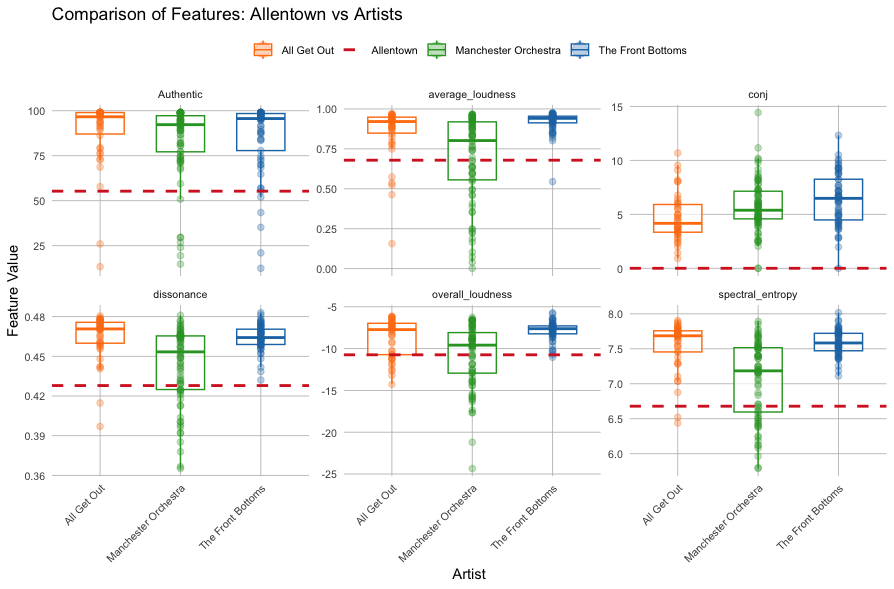
\includegraphics[scale=0.8]{figure/Rplot.png}
\label{plot1}
\end{center}
\end{figure}

\section{Bibliography}
 @Manual{xtable,
title = {xtable: Export Tables to LaTeX or HTML},
author = {David B. Dahl and David Scott and Charles Roosen and Arni Magnusson and Jonathan Swinton},
year = {2019},
note = {R package version 1.8-4},
url = {https://CRAN.R-project.org/package=xtable},
}
@inproceedings{bogdanov2013essentia,
  title={Essentia: An audio analysis library for music information retrieval.},
  author={Bogdanov, Dmitry and Wack, Nicolas and G{\'o}mez, Emilia and Gulati, Sankalp and Herrera, Perfecto and Mayor, Oscar and Roma, Gerard and Salamon, Justin and Zapata, Jos{\'e} Ricardo and Serra, Xavier and others},
  booktitle={ISMIR},
  volume={13},
  pages={493--498},
  year={2013}
}
\end{multicols}

\end{document}
